\documentclass{article}

\usepackage{amssymb}
\usepackage{amsfonts}
\usepackage{amsmath}
\usepackage[margin=1in]{geometry}
\pagestyle{empty}

\newtheorem{thm}{Theorem}[section]
\newtheorem{conj}[thm]{Conjecture}
\usepackage{graphicx}
\usepackage{epstopdf}
\usepackage{wrapfig}
\usepackage{float}
\begin{document}	
\noindent 80977816 \hspace{5.5in} 3/28/17\\

\begin{enumerate}
	\item The probability that if there are $m$ people and $n$ possible hashes, that no two people have the same half can be expressed as $\displaystyle\prod_{i = 0}^{m-1}(1-\frac{i}{n}) = 1(1 - \frac{1}{n})(1-\frac{2}{n})...(1 - \frac{m-1}{n})$, assuming that $m \leq n$, otherwise the probability is 0.  This is just a slight generalization of the birthday paradox discussed in lecture.  Now using the inequality $1 - x \leq e^{-x}$ we can see that this probability is bounded by: \\\\
	$e^{-1/n}e^{-2/n}...e^{-(m-1)/n} = e^{\frac{-m(m-1)}{2n} }$. \\
	Now because we want to find the value for $c_1$ such that when there are at least $c_1\sqrt{n}$ people the probability that no two have the same hash value is at most $e^{-1}$,  so we say that $m = c_1\sqrt{n}$ and so \\\\
	$e^{-c_1\sqrt{n}(c_1\sqrt{n} - 1) / (2n)} \leq e ^{-1}$ \\
	$c_1^2n - c_1\sqrt{n} \geq 2n$ \\
	$\sqrt{n}c_1^2 - c_1 - 2 \sqrt{n} \geq 0$ \\
	$c_1 = \dfrac{1 + \sqrt{1 + 8n}}{2 \sqrt{n} }$ which as $n$ gets sufficiently large, $c_1$ approaches $\sqrt{2}$.  For $n = 2$, $c_1 \approxeq 1.81$, and for $n\geq 36$, $c_1 \leq 1.5$ in order for these conditions to be maintained.  Of course, $c_1$ can be made even larger than these values that the constraints will still hold. \\
	
	Now, continuing for $c_2$ we start with a similar inequality.  \\
	
	\[ (1 - \frac{1}{n})(1-\frac{2}{n})...(1 - \frac{c_2\sqrt{n}-1}{n})\geq \frac{1}{2} \]
	
	Assuming $n$ is large enough such that $\frac{c_2\sqrt{n}-1}{n}\leq \frac{1}{2}$ then we can use the second inequality to come up with a bound for $c_2$ in this way: \\
	
	\[ (1 - \frac{1}{n})(1-\frac{2}{n})...(1 - \frac{c_2\sqrt{n}-1}{n}) \geq e^{-\frac{1}{n} - \frac{1}{n^2}}e^{-\frac{2}{n}-\frac{4}{n^2}}...e^{-\frac{c_2\sqrt{n} - 1}{n} - \frac{(c_2\sqrt{n} - 1)^2}{n^2}} \geq \frac{1}{2} \]
	Using the fact that the sum of the first $n$ numbers is $\frac{n(n+1)}{2}$ and that the sum of the first $n$ squares is $\frac{n(n+1)(2n+1)}{6}$ we see that, \\
	\[e^{-\frac{c_2\sqrt{n}(c_2\sqrt{n} - 1)}{2n} - \frac{c_2\sqrt{n}(c_2\sqrt{n}-1)(2c_2\sqrt{n} - 1)}{2n^2}} \geq \frac{1}{2} = e^{-\ln2} \] \\
	
	\[-\frac{c_2\sqrt{n} (c_2\sqrt{n} - 1) }{2n} - \frac{c_2\sqrt{n}(c_2\sqrt{n}-1)(2c_2\sqrt{n} - 1)} {2n^2} \geq -\ln2 \] \\

	And after much simplifying, we get: \\
	
	\[-2c_2^3 - c_2^2n^2 + 3c_2^2n+c_2n^{3/2} - c_2\sqrt{n} + 2n^2\ln2 \geq 0 \]
	
	Dropping the lower order terms,\\
	
	\[-c_2^2n^2+2n^2\ln2 \geq 0 \]
	\[\sqrt{2\ln2} \geq c_2 \]


	\item Using $k$ hash functions and $m$ total locations there are $m / k$ locations per hash table.  Therefore, the probability that an element is hashed to a particular location is equal to $\frac{k}{m}$.  Consequently, if there are $n$ elements, then the probability that $i$ elements get hashed to that one counter is ${n \choose i}(\frac{k}{m})^i\cdot (1 - \frac{k}{m})^{n - i}$.  \\\\
	So if a $b$ bit counter is being used then that counter will overflow only when there are more than $2^{b} - 1$ elements hashed to it.  \\
	P(no overflow on $b$ bits) = $\displaystyle\sum_{i = 0}^{2^b - 1} {n \choose i} (\frac{k}{m})^i\cdot (1 - \frac{k}{m})^{n - i}$ \\\\
	The probability of overflowing on $b$ bits = $1 - P($no overflow on $b$ bits$)$. \\
	Using $n = 10^5, m = 10^6, k = \lceil m / n \cdot \ln2 \rceil = \lceil 10 \ln 2 \rceil = 7$, and letting $b = 3$ I found that the probability of a counter overflowing is approximately $7.69 \cdot 10^{-7}$.  For a 4 bits, I found this probability was roughly $1.11 \cdot 10^{-16}$ and for 5 bits $7.88\cdot 10^{-41}$.   Therefore given these values for $k,m,$ and $n$ it seems that a 4 bit counter should be sufficient.  
	
	\item If using a 64-bit hash function the probability that two documents will agree when they don't agree on all 14 of the corresponding values is $\frac{1}{2^{64}}$ because this is a perfectly random hash function.  However, in practice this probability is so small we can ignore it and so it is safe to say that the only time there will be a match on the super sketch values is when all 14 values between two documents actually agree. \\
	Therefore, if two documents have resemblence $r$ then per the arugments discussed in lecture, the probability that they agree on one of the 84 permutations is $r$ and given what was just said, the probability that they agree on all 14 of a given group and thus, there's a match within the super sketch is $r^{14}$.  \\
	
	Thus $P(\geq 2$ matches$) = 1 - P(0$ matches$) - P(1 $match$) = 1 - (1 - r ^{14})^6 - {6 \choose 1}(1 - r^{14})^5r^{14}$, which assumes there are no hash collisions or rather that the probability of a collision is so insignificant we can disregard it. Below is a graph over this probability vs $r$.  As you can see it's not until the resemblence exceeds 90\% that there's an even 50 percent chance that there are more than 2 matches on the super sketches.  \\
	
	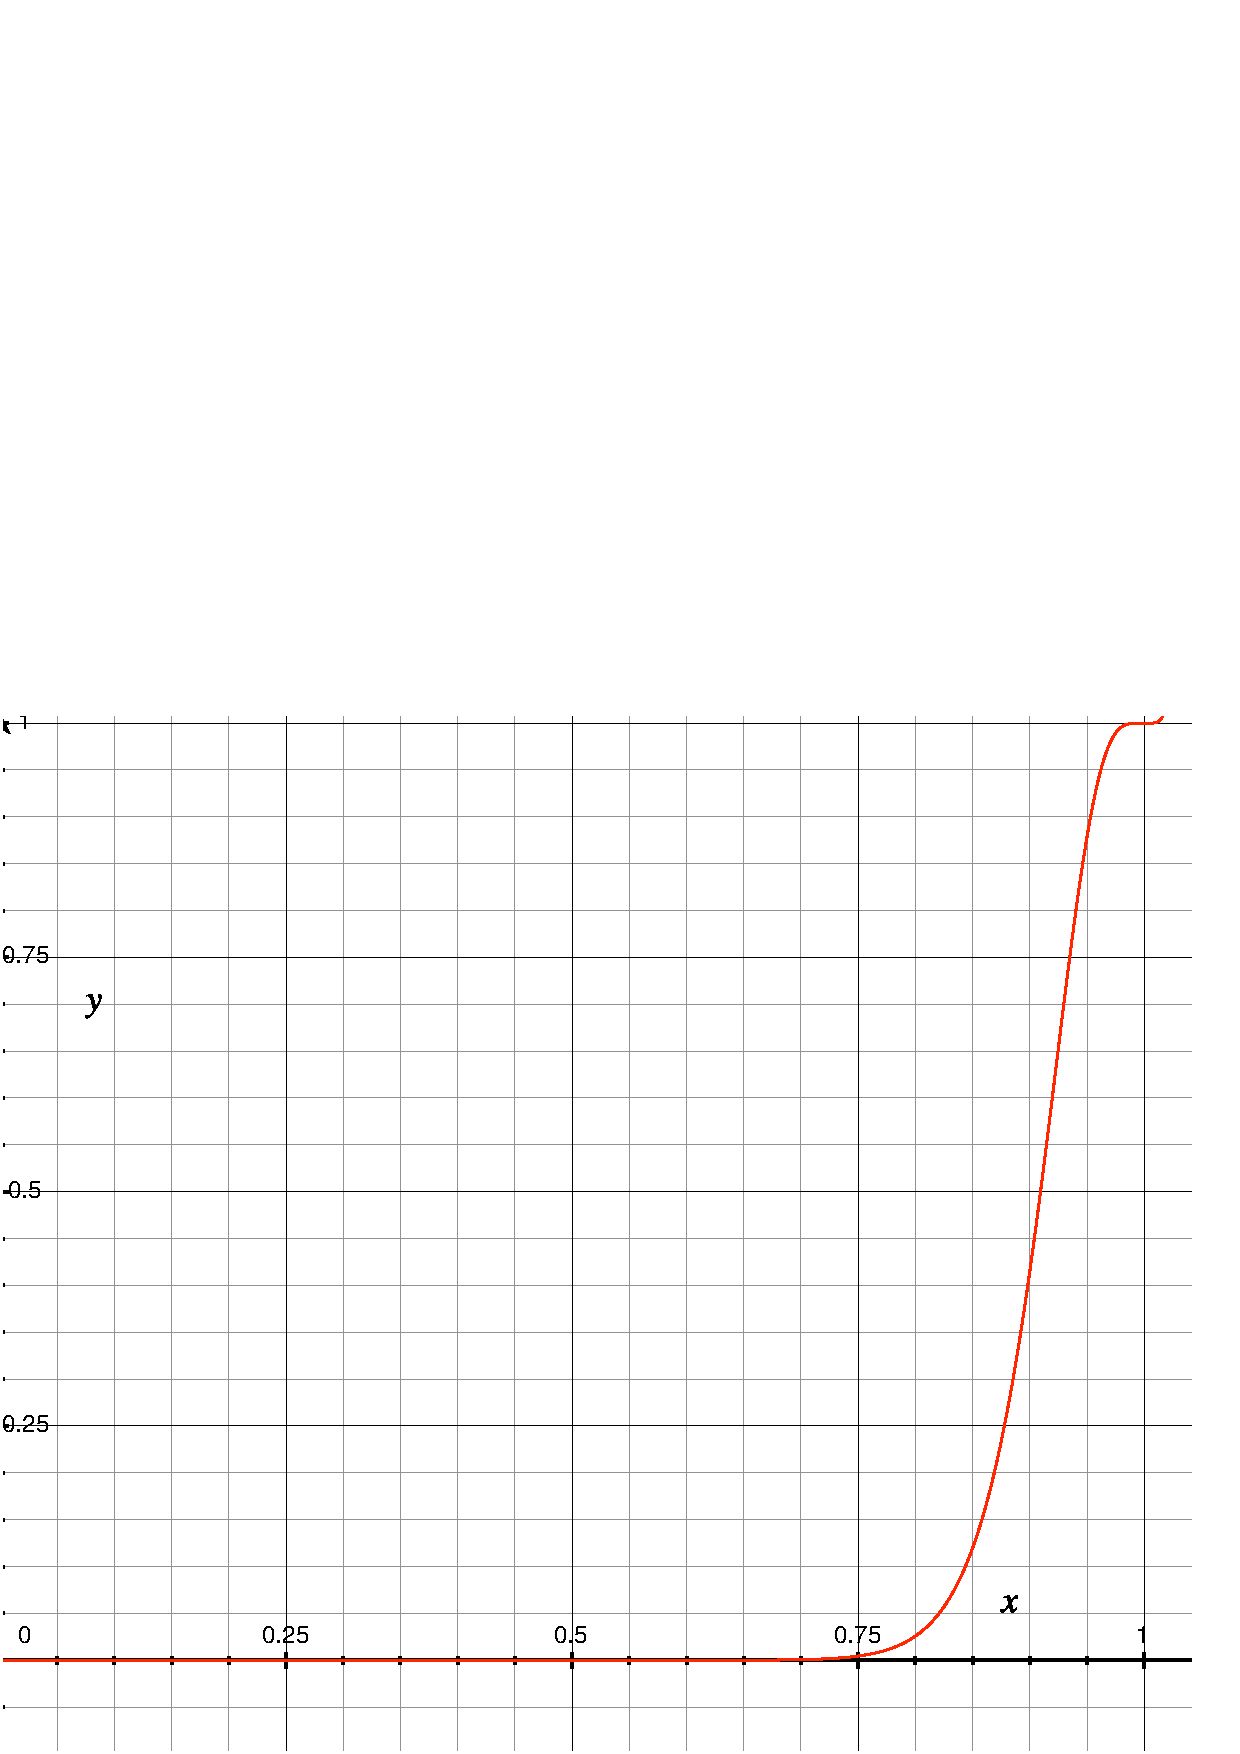
\includegraphics[width=0.5\textwidth]{Graph_Question_3.pdf}
	\\
	
	If a 16 bit or 8 bit hash function were used instead the probability of a collision would rise to $\frac{1}{2^{16}}$ and $\frac{1}{2^8}$ respectively and this values may be large enough that they should be factored into the calculations for a match.  \\
	
	Again, $P(\geq 2 $matches on 6 sketches ) = $1 - P(0 $ matches$) - P(1 $ match$)$. However the possibility of a hash collision changes these probabilities. These probabilities are calculated if a $b$-bit hash were used  \\
	$P(0$ matches) = $((1 - r^{14})(1 - \frac{1}{2^b}))^6$ because the probability that one of the values of the sketch differs between the two documents is the probability that at least one of the values in the group of 14 that generated that value is different which is $(1 - r^{14})$ times the probability that there's no hash collision which is $(1 - \frac{1}{2^b})$ and because there are 6 values in the sketch this is raised to the 6th power.  \\
	$P(1$ match) = ${6\choose 1}((1 - \frac{1}{2^b})(1 - r^{14}))^5(r^{14} + \frac{1}{2^b}(1 - r^{14}))$ which is valid because first we pick one of the groups to match and the other five do not match and this group that matches can match either because all 14 values are the same or becuase they don't match and there's a hash collision.  \\
	So, using a $b$ bit hash, $P(\geq 2$ matches) = $1 - ((1 - r^{14})(1 - \frac{1}{2^b}))^6 - {6\choose 1}((1 - \frac{1}{2^b})(1 - r^{14}))^5(r^{14} + \frac{1}{2^b}(1 - r^{14}))$ \\
	
	\item First off, I'm assuming that all $k$ patterns are the same length - this was discussed on Piazza.  In order not to increase the runtime of this pattern matching by a factor of $k$ and to do it wiht just one pass through the document, at every shingle we come across (as described in the fingerprinting lecture), instead of just comparing that value to  one pattern, compare it to all $k$ patterns to see if there's a match.  Because the bulk of the computation for this problem is spent computing the fingerprints, this will not increase the runtime significantly  Because every shingle is checked against $k$ values, the probability of a false positive match occuring has now increased by a factor of $k$.  So the probability of a false positive at any given step is $\dfrac{k\cdot \log_210^{|P|}}{\pi(Z)}$ and the overall probability of a false match anywhere is at most $|D|$ times this probability. The expected number of false positives is $k$ times what it would be if we were searching for only one pattern. \\
	
	Another solution that would have the same asymptotic running time, but would only involve one comparison at each step can be done if we create a hash table for all of the $k$ patterns we're trying to match.  First, we hash the $k$ patterns into some table, using the same hash function we'd use on the document.  Every time we have a shingle in the document we check if its hash is in the table and if it is, it's very likely a match.  Of course, the one thing we won't know if we search for patterns this way is how many of each pattern we find, just how many matches.  The probability of a false positive at any given step remains the same as it did when we made $k$ comparisons, but now we do that with a constant lookup.   
	
	\item Because 636127 is not a Carmichael number, we can use Fermat's little theorem to determine whether or not it is a prime number.  Fermat's test says that for some $a$, if $a ^ {n-1} \not\equiv 1$ mod $ n$, then $n$ is not a prime number.  I found that 2 is a witness for the fact that 636127 is composite because $2 ^ {636126} \equiv 195504$ mod $ 636127$ which demonstrates that 636127 is composite. It turns out that 636127 = 617 * 1031 and so it is definitely not prime. \\
	
	Because 294409 is a Carmichael number then for all $a$ relatively prime to 299409, $a^{299408}$  mod  $299409$ will be one even though 299409 is a composite number - 3 is clearly a factor.  Therefore, instead of Fermat's primality test which would tell us that 294409 is probably prime, we can use the Rabin-Miller randomized primality algorithm discussed in class to demonstrate that this is prime.  \\
	Upon running Rabin-Miller, it turns out that $a = 124410$ is a witness.  Let $n = 299409$ and note that $n - 1 = 299408 = 2 ^ 3 \cdot 36801$.  Ultimately we need to calculate $a ^ {n - 1}$ mod $n$ via repeated squaring and if at any point we find a nontrivial square root modulo $n$ then we can conclude that $n$ is composite because having a nontrivial square root implies compositeness.  So going through the steps of the algorithm, we see that $a^{36801} = 207830$ mod $n$, $27830 ^ 2 = 270101$ mod $n$, and finally that $270101 ^ 2 = 1$ mod $n$ and therefore 270101 is a square root of 1 mod $n$ and because 270101 does not equal 1 or $n - 1$ it is nontrivial and therefore $n$ is composite. 
	
	\item The string "Give me an A" encoded with this public key is 27016764340118192395712492378.  See the code in problem5\_6.py to see how this was calculated.  
	
	\item I'm calling part a to be the first experiment in which bins are drawn one at a time and a bal is placed into it and part b is the part in which two bins are selected each trial and the one with fewer balls currently gets a ball placed in it.  
	
	\begin{tabular}{l | c | r}
	Trial & Max Load A & Max Load B \\
	\hline
	1 & 11 & 4 \\
	2 & 11 & 4 \\
	3 & 11 & 4 \\ 
	4 & 11 & 4 \\
	5 & 12 & 4 \\
	6 & 11 & 4 \\
	7 & 11 & 4 \\
	8 & 11 & 4 \\
	9 & 12 & 4 \\
	10 & 12 & 4 \\	
	\end{tabular}
	
	So in order to calculate these values without keeping track of an array of size $10^9$, I used an array called counts of size of 25 in which counts$[i]$ would give the number of bins that had $i$ balls in them currently.  It is safe to assume that no more than 25 spaces will be needed (and 25 is likely overkill for only a billion balls and bins) because the probability that $L$ of the $n = 10 ^ 9$ balls ends up in any particular bin is equal to ${n\choose L}(\frac{1}{N})^L(1 - \frac{1}{N})^{N-L}$ which by the Poisson approximation with $\lambda = np = n \cdot \frac{1}{n} = 1$ is very nearly equal to $\frac{1}{e}\cdot\frac{1}{L!}$.  This, of course, gives the probability that a particular bin has $L$ balls not that any bin does - so while it is not an exact probability it gives a sense of how likely it is for a bin to have $L$ balls and let me set a cap on the number of bins to keep track of.  In practice as demonstrated by the second column in that table the max wasn't larger than 12 and for the second half in which balls are distributed semi-randomly there were never more than 4 bins in any ball.  \\
	
	This is how I did the simulation. I started by initializing counts[0] to $10^9$ and then I generated a random number between 0 and $10^9 - 1$ which would correspond to the number of the bin I needed to update.  Because the built in rand() function generates a number between 0 and $2^{31}$ which is approximately 2.1 billion, using this function if taken mod $10^9$ disproportionately selects a number that will correspond to one of the first 100 million numbers and so instead of using that I found a C program called Mersenne Twister that generates 64 bit integers (which is suitably large for $10^9$) to generate these numbers instead.  To see that this skewing actually occurs, look at bad\_rand.txt - if generated randomly there should be approximately the same number of bins that have 0 balls and 1 ball in them, but that's not the case.  \\
	
	Anyway, once you have a random number, that corresponds to the bin a ball is going to be added to.  I'm treating the array counts[] as a compact, order list of the bins such that if counts (for a smaller $n$) looked like [5, 3, 2, 0, 0], then the first 5 bins would have 0 balls, the next 3 would have 1, and the last 2 would have 2.  So if 6 were generated, bin 6 currently has 1 ball in it, I would decrement counts[1] by 1 and increment count[2] by 1 and continue this process $10^9$ times.  \\
	
	For part $b$, instead of generating a random number modulo $10^9$, generate two numbers and return whichever one is smaller.  By the construction of counts[] this always corresponds the smaller of the two numbers always leads a bin that has at most as many balls as the other bin.  \\
	
	For part a, it seems that the maximum load, at least for $10^i, i = 2...10$ grows at a rate very close to $O(logn)$ because the average maximum load roughly increases by 1 every time the number of bins and balls is multiplied by 10, but not exactly.  
	
	For part b, for values of $n$ less than $10^6$, is less than 4 but for values larger than $10^6$ it seems to consistently be 4 and I couldn't find a large enough value that would make the maximum load 5, so this value grows much more slowly than the load for part a. 
	
	
\end{enumerate}

	\newpage I collaborated with Manav Khandelwal and Lauren Kim on this assignment.  
\end{document}
